This section will describe the basic design of the \nenwin scheme. Note that \nenwin represents a class of algorithms, similar to neural networks: each network encodes a different algorithm, but the underlying mechanics are the same. Here the underlying mechanics of \nenwin will be explained.

\subsection{Objects}
\nenwin is best described by defining a family of objects known as particles. The scheme uses a subspace of $\mathbb{R}^n$, often $n=2$ is used in this report to support visualizations, but any higher dimensionality can be used as well. Each particle has a position, a velocity and an acceleration, which are all vectors in $\mathbb{R}^n$. Each particle has a mass (i.e. a decimal value, \textit{allowed to be negative}) as well, and its acceleration is at any point in governed by Newton's Second Law \cite{principia} and a force vector $\vec{f}$:
\begin{equation}
    p.acc = \frac{1}{p.mass} \sum_{\vec{f} \text{ acting on } p}\vec{f}
\end{equation}
Where $p.acc$ and $p.mass$ are the acceleration and mass of any particle $p$.

Note that these forces can only be caused by other particles. Each particle has an associated \textit{attraction function}, that describes what force the particle exerts on any other particle. Although many different functions can be used for this purpose, a natural first choice would be the gravity function (with the constant factor $G$ (the gravitational acceleration) replaced by 1):
\begin{equation}
    \norm{\vec{f}} = \frac{p_1.mass \cdot p_2.mass}{\norm{p_1.pos - p_2.pos}^2}. \label{eq:newton_grav_force}
\end{equation}
The direction of the force is the direction from the first particle to the second particle, so the force vector is given by:
\begin{equation}
    \vec{f} = \frac{p_1.pos - p_2.pos}{\norm{p_1.pos - p_2.pos}} \cdot\frac{p_1.mass \cdot p_2.mass}{\norm{p_1.pos - p_2.pos}^2}. \label{eq:newton_grav_force}
\end{equation}

Particles are divided into two general subclasses: Nodes and Marbles. Nodes are used to represent an architecture, they are the fixed part of a \nenwin network that encodes an algorithm. Nodes are further subdivided into MarbleEaterNodes and MarbleEmitterNodes, as described later. Marbles represent input and output data, and are created at runtime. Marbles can keep an optional reference to the datum they represent.

Particles \textit{experience} forces exerted on them by other particles, but also \textit{exert forces onto} other particles. Unlike in classical mechanics, \nenwin does not require these forces to be symmetric. 
To regulate the \textit{experienced} forces, each particle $p$ has the attributes \texttt{marble\_stiffness} and \texttt{node\_stiffness}. These act as multipliers for experienced forces, and are required to be real values in $[0, 1]$.
The forces that each particle $p$ exerts onto other particles, is regulated in a similar way: $p$ has two attributes\texttt{marble\_attraction} and \texttt{node\_attraction}, act as multipliers of the force that $p$ exerts onto other particles. Also these attributes must be real values in $[0, 1]$. 

To summarize, the motion of a particle $p$ is described by the following differential equations:
\begin{align}
    &p.pos = p.pos_0 + \nabla p.pos \cdot t  = p.pos_0 + p.vel \cdot t \label{eq:def_pos} \\
    &p.vel = p.vel_0 + \nabla p.vel \cdot t = p.vel_0 + p.acc \cdot t \label{eq:def_vel}\\
    &\vec{f}_{net}  = \texttt{marble\_stiffness} \cdot \sum_{\text{Mables $m$ acting on $p$}} \frac{p.mass \cdot m.mass}{\norm{p.pos - m.pos}^2} \nonumber \\
    & \qquad + \texttt{node\_stiffness} \cdot \sum_{\text{Nodes $n$ acting on $p$}} \frac{p.mass \cdot n.mass}{\norm{p.pos - n.pos}^2} \label{eq:def_f_net}\\
    &p.acc = \frac{\vec{f}_{net}}{p.mass} \label{eq:def_acc}
\end{align}
Where $t$ denotes the amount of time passed, and $p.pos_0$ and $p.vel_0$ the initial position and velocity respectively of the particle when it was created.
The acceleration of $p$ depends the forces $p$ experiences. These forces are a function of $p$'s relative distances to other Marbles and Nodes (the denominators in \eqref{eq:def_f_net} are distance measures). These distances depend on the value of $p.pos$ and the motion of other particles. Hence $p.pos$, $p.val$ and $p.acc$ are highly dependent on the other particles in a \textsc{Nenwin} model, and can change significantly even when only an very small amount of time passes.

To enable output production, a special subclass of Node called the MarbleEaterNode is used: this class stores an additional real-valued radius. When, in the simulation, the distance between a Marble and a MarbleEaterNode becomes smaller than the radius of the MarbleEaterNode, then the Marble will be removed from the simulation: it was 'eaten' by the MarbleEaterNode. The MarbleEaterNode keeps both a count of the amount of Marbles consumed, and a set of references to the associated data of the consumed Marbles.

\subsection{Motivation Emitter Nodes}
\nenwin will have a nonincreasing amount of particles if only Marbles, Nodes and MarbleEaterNode would be used.
Marbles can be removed when eaten by a MarbleEaterNode, but the there is no internal way the system can produce new Marbles (other than awaiting new input).
This would imply that the amount of information that can be stored in a \nenwin simulation is also nonincreasing in a \nenwin architecture.

Turing Machines, on the other hand, can \textit{increase} the information stored on their tape. As a simple example, consider a simple Turing Machine that has only a single state, writes the same symbol (e.g. '1') every step, and moves the head left every step. If this machine is given an blank tape (i.e. all cells contain the empty symbol '$\Box$'), and set to run for $n \rightarrow \infty$ steps, then the resulting tape will approach a tape with half (the cells left of the starting position) of the cells blank, and the other half carrying the symbol '1'. The entropy of the blank tape is 0, as the probability that a cell is blank is 1. The tape will approach an entropy of $\infty$ when $n \rightarrow \infty$, as for each tape cell with index $i$ we have:
\begin{equation}
    entropy(Tape[i]) = -\sum_{x \in \{\Box, 1\}}p(Tape[i] == x)\cdot\log_2(p(Tape[i] == x)) = 1
\end{equation}
As there are infinite tape cells, the entropy of the whole tape will approach $\infty$. Hence a Turing Machine can create any arbitrary amount of entropy in its 'working memory'.

The \nenwin scheme so far described is not able to create any arbitrary amount of entropy. There is only a finite amount of information (and hence entropy) that can be encoded in a finite set of particles.

\subsection{EmitterNode}
To make \nenwin able to create more entropy, we add an additional Node called an EmitterNode \footnote{or, more specifically, a MarbleEaterNode. Note that there is no theoretical objection against creating EmitterNodes that emit other Nodes, other than the fact that EaterNodes cannot eat each other.}. This Node will create another particle at its own position when a certain condition is met.

There are many different ways to choose the exact behavior of EmitterNodes, but in this paper we use the following:
\begin{itemize}
    \item An EmitterNode is a special case of a MarbleEaterNode, and tracks also the cumulative mass of Marbles it has consumed in a field \texttt{stored\_mass}.
    \item The EmitterNode can only create Marbles with predefined parameters (mass, initial velocity, etc.) at its own position.
    \item At a fixed time interval, the EmitterNode will create a new Marble and subtract its mass from \texttt{stored\_mass}, unless \texttt{stored\_mass} is smaller than the mass of the would-be created Marble. \\
    In case the mass of the Marble is negative, it will only be created as long as the \texttt{stored\_mass} is \textit{at most} the value of the mass of the Marble (i.e. also negative with a magnitude at least as great as the mass of the Marble).
    \item The created Marble must be within the radius or at an infinitesimal distance from the border of the radius of the EmitterNode. In case the Marble is within the radius it will be consumed immediately, hence only the infinitesimal distance is practical. In implementation, where infinitesimal numbers cannot be represented, a small constant $\epsilon$ can be defined such that we require (if $emitter$ is the EmitterNode that creates Marble $m$):
    \begin{align}
        \epsilon > 0 \quad \land \quad distance(emitter.pos, m.pos) \leq emitter.radius + \epsilon
    \end{align}
\end{itemize}

To see how EmitterNodes can be used to create any arbitrary amount of entropy, consider an EmitterNode that generates Marbles with infinitesimally small mass, or even 0 mass. After eating a Marble with a finite mass, it will be able to generate infinitely many new Marbles. Each of these new Marbles can take on a unique positions, if a dynamic system guides their movement, since they are not created at the same moment. Hence an infinite entropy can be created.

See \ref{fig:particles_class_diagram} for a diagram the complete particle hierarchy. 

\begin{figure}[h]
    \centering
    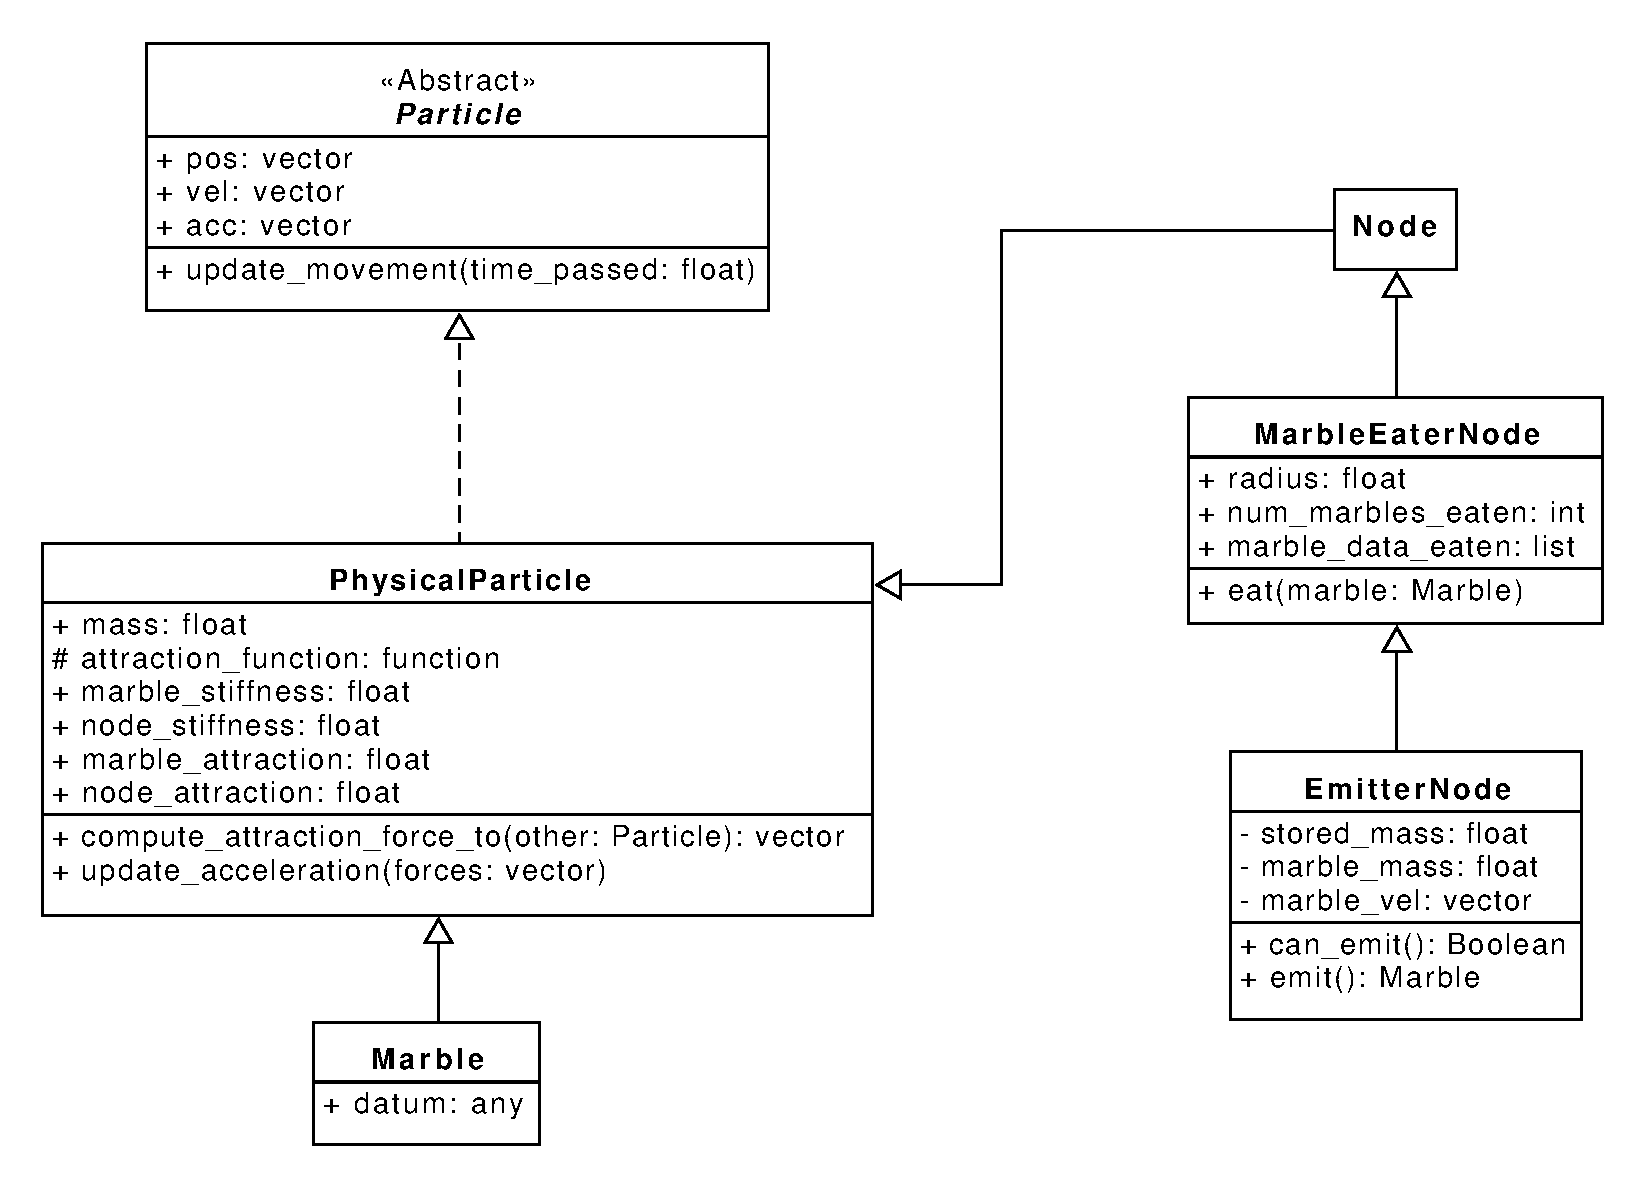
\includegraphics[scale=0.5]{figures/particles_class_diagram.pdf}
    \caption{UML class diagram depicting the inheritance relations between different particles. Note that the exact inheritance and attribute-visibilities may vary between implementations. For example, in the provided implementation, Marble is a subclass of Node.}
    \label{fig:particles_class_diagram}
\end{figure}

\subsection{Particle attributes}
An overview of the different attributes per particle subclass is given in Table \ref{table:attributes} 

\begin{table}[h]
\begin{tabular}{llllll}
\textbf{Attribute} & \textbf{type} & \textbf{Marble} & \textbf{Node} & \textbf{MarbleEaterNode} & \textbf{EmitterNode} \\ \hline
\multicolumn{1}{l|}{\texttt{pos}}                  & \multicolumn{1}{l|}{$\mathbb{R}^n$} & \checkmark & \checkmark & \checkmark & \checkmark \\
\multicolumn{1}{l|}{\texttt{vel}}                  & \multicolumn{1}{l|}{$\mathbb{R}^n$}               & \checkmark & \checkmark & \checkmark & \checkmark \\
\multicolumn{1}{l|}{\texttt{acc}}                  & \multicolumn{1}{l|}{$\mathbb{R}^n$}               & \checkmark & \checkmark & \checkmark & \checkmark \\
\multicolumn{1}{l|}{\texttt{marble\_stiffness}}    & \multicolumn{1}{l|}{{[}0, 1{]}}     & \checkmark & \checkmark & \checkmark & \checkmark \\
\multicolumn{1}{l|}{\texttt{node\_stiffness}}      & \multicolumn{1}{l|}{{[}0, 1{]}}     & \checkmark & \checkmark & \checkmark & \checkmark \\
\multicolumn{1}{l|}{\texttt{marble\_attraction}}   & \multicolumn{1}{l|}{{[}0, 1{]}}     & \checkmark & \checkmark & \checkmark & \checkmark \\
\multicolumn{1}{l|}{\texttt{node\_attraction}}     & \multicolumn{1}{l|}{{[}0, 1{]}}     & \checkmark & \checkmark & \checkmark & \checkmark \\
\multicolumn{1}{l|}{\texttt{attraction\_function}} & \multicolumn{1}{l|}{$f:\mathcal{P}\times\mathcal{P}\rightarrow \mathbb{R}^n$}       & \checkmark & \checkmark & \checkmark & \checkmark \\
\multicolumn{1}{l|}{\texttt{datum}}                & \multicolumn{1}{l|}{any object}     & \checkmark &   &   &   \\
\multicolumn{1}{l|}{\texttt{eaten\_marbles}}       & \multicolumn{1}{l|}{stack of Marbles} &   &   & \checkmark & \checkmark \\
\multicolumn{1}{l|}{\texttt{radius}}               & \multicolumn{1}{l|}{$\mathbb{R}$}           &   &   & \checkmark & \checkmark \\
\multicolumn{1}{l|}{\texttt{stored\_mass}}       & \multicolumn{1}{l|}{$\mathbb{R}$} &   &   & \checkmark & \checkmark \\
\multicolumn{1}{l|}{\texttt{spawnpos}}             & \multicolumn{1}{l|}{$\mathbb{R}^n$}            &   &   &   & \checkmark \\
\multicolumn{1}{l|}{\texttt{prototype\_marble}}    & \multicolumn{1}{l|}{Marble}         &   &   &   & \checkmark
\end{tabular}
\caption{A summary of different attributes used by different particles. $\mathcal{P}$ is used to denote the set of all particles in a given architecture. Here \texttt{pos}, \texttt{vel} and \texttt{acc} are the position, velocity and acceleration of a particle, which are real vectors defined in $\mathbb{R}^n$ where $n$ is the dimensionality of the architecture. The stiffness and attraction values are real numbers in the interval $[0, 1]$. The attraction function maps two particles to a vector of the same shape as \texttt{acc}. The \texttt{datum} is any data-element that a Marble represents, and this attribute is allowed to be valueless. \texttt{eaten\_marbles} is a stack of all Marbles a MarbleEaterNode (or its subclass, a MarbleEmitterNode) has consumed, with the latest consumed Marble on top of the stack. This stack is allowed to be empty. The \texttt{radius} of a MarbleEaterNode is the maximum distance such that, if a Marble is at this distance or at a smaller distance to the MarbleEaterNode, it will be consumed. The \texttt{stored\_mass} is the cumulative mass of the Marbles in \texttt{eaten\_marbles} of a MarbleEmitterNode, minus the cumulative mass of emitted Marbles. This value is allowed to be negative, which is required to emit negatively-massed Marbles. The \texttt{spawnpos} is the relative position from the center of an MarbleEmitterNode at which a Marble can be created when emitted, this point is at most \texttt{radius} + $\varepsilon$ away from the center of the MarbleEmitterNode, where $\varepsilon$ is an infinitesimal number. The prototype Marble is a 'blueprint' of the Marble that is emitted: all its attributes are copied to a new Marble that is being emitted, except the position (which is governed by the combination of the position of the MarbleEmitterNode and \texttt{spawnpos}), the velocity and the acceleration (which are set to $\vec{0}$).}
\label{table:attribute}
\end{table}

\clearpage
\subsection{Pseudocode}
See Algorithm \ref{alg:Nenwin_V1} below for a pseudo-code description how a \nenwin network is being simulated. Note that in implementation the functionality will be subdivided into different modules. It is for example equally fast, but from an Object-Oriented point of view preferable, to first create Marble instances for new inputs and then sending them over the channel rather than sending the raw data itself.

\begin{algorithm}[h]
	\label{alg:Nenwin_V1}
	\caption{\\\textsc{Nenwin}\textnormal{\texttt{(nodes, input\_space, placement\_function, mass\_function, channel, attraction\_function)}}}
	\newcommand{\dataStyle}[1]{\textbf{\texttt{#1}}}
	\SetAlgoLined
	\SetKwSty{texttt}
	\SetDataSty{dataStyle}
	% Setup variables
	\SetKwData{nodes}{nodes}
	\SetKwData{input}{input\_space}
	\SetKwData{placement}{placement\_function}
	\SetKwData{channel}{channel}
	\SetKwData{node}{Node}
	\SetKwData{grav}{attraction\_function}
	\SetKwData{mass}{mass\_function}
	\SetKwData{eaters}{eater\_nodes}
	\SetKwData{emitters}{emitter\_nodes}
	% Input and output
	\KwIn{
		\nodes: A set of \node objects, each having a position, velocity and acceleration in $\mathbb{R}^n$ and a stiffness and a mass in $\mathbb{R}$.\\
		\input: A rectangular region of $\mathbb{R}^n$.\\
		\placement: A function: $\mathbb{N} \rightarrow \input$ that maps the index of an element in input to a position in \input.\\
		\mass: A function: $object \rightarrow \mathbb{R}$ that maps any datum to a mass-value.\\
		\channel: A bi-directional communication channel (of finite capacity) over which any finite bit sequences can be sent.\\
		\grav: A function: $\mathbb{R}^3 \rightarrow \mathbb{R}$ that maps the masses of two particles plus their distance to an attraction force.		
	}
	\KwOut{\texttt{None}}
	$particles \leftarrow \nodes$ \;
	$\eaters \leftarrow [node: node \in \nodes \land node \text{ is a } \textsc{MarbleEaterNode}]$ \;
	\tcc{The following is a subset of 'eaters':}
	$\emitters \leftarrow [node: node \in \nodes \land node \text{ is a } \textsc{MarbleEmitterNode}]$ \;
	\While{\texttt{True}}{
		\If{there is input on the channel}{
			\For{$(object, index) \in \channel$}{
				$position \leftarrow \placement(index)$ \;
				$mass \leftarrow \mass(object)$ \;
				$velocity \leftarrow \vec{0}$ \;
				$acceleration \leftarrow \vec{0}$ \;
				$node\_stiffness, marble\_stiffness, marble\_attraction \rightarrow 0$ \;
				$node\_attraction \rightarrow 1$ \;
				$particles \leftarrow particles \cup \{\texttt{Marble}(position, velocity, acceleration, mass, $
				$node\_stiffness, marble\_stiffness, marble\_attraction, node\_attraction)\}$
			}
		}
		\If{there is an output request on the channel}{
			$output \leftarrow \text{ a new empty list}$ \;
			\For{$node \in \eaters$}{
			    $output.append(node.num\_marbles\_eaten)$ \;
			}
			Place $output$ on the channel \;
		}
		\For{$particle \in particles$}{
			$forces \leftarrow 0$ \;
			\For{$other \in particles \setminus \{particle\}$}{
				$difference \leftarrow other.pos - particle.pos$ \;
				$direction \leftarrow \frac{difference}{\norm{difference}}$ \;
				$forces += direction \cdot \grav(particle.mass, other.mass, \norm{\norm{difference}})$
			}
			\tcc{Newton's Second Law}
			$particle.acc \leftarrow particle.mass \cdot forces$ \;
		}
		\For{$emitter \in \emitters$}{
		    \If{$\norm{emitter.stored\_mass} \geq \norm{emitter.prototype\_marble.mass} \land \sgn{emitter.stored\_mass} = \sgn{emitter.prototype\_marble.mass}$}{
		    $particles \leftarrow particles \cup (\text{a copy of $emitter.prototype\_marble$ at position $emitter.pos + emitter.spawnpos$})$
		    }
		}
		\For{$particle \in particles$}{
			Numerically compute and update $particle$'s next position and velocity given their current acceleration. \;
		}
		$\dots$ \;
		}
\end{algorithm}

\begin{algorithm}
    \setcounter{AlgoLine}{30}
    \SetKwData{eaters}{eater\_nodes}
    \SetKwBlock{Begin}{$\dots$}{end}
    
    \SetAlgoVlined
    \SetAlgoLined
    \Begin{\For {$marble \in particles \setminus nodes$}{
		    \For{$node \in \eaters$}{
			    \If{$distance(marble.pos, node.pos) \leq node.radius$}{
			        $particles \leftarrow particles \setminus \{marble\}$ \;
			        $node.stored\_mass \leftarrow node.stored\_mass + marble.mass$ \; $node.eaten\_marbles \leftarrow node.eaten\_marble \cup \{marble\}$\;
			        }
			    }
			    }
		}
\end{algorithm}
\clearpage